% TPCU 碩士學位論文 LaTex 樣板
% 使用 utf-8 編碼
% v0.5 (Jun. 30, 2012)
% by Peter

\documentclass[a4paper,12pt]{report}


% 引用必要的套件
\usepackage{tpcu}ls
\usepackage{tikz}
\usetikzlibrary{shapes,arrows}
\usepackage[english]{babel}
\usepackage{blindtext}

%\usepackage{chap_last}

\usepackage{xcolor,tikz}
%\usepackage[usenames,dvipsnames,pdftex]{xcolor}
%\def\pgfsysdriver{pgfsys-dvipdfmx.def}
%\usepackage{tikz,ifthen}

\newcommand{\newchapter}[1]{%
    \chapter{#1}
%   \pagestyle{fancy}
    \thispagestyle{fancy}
%   \fancyhead[LO,RE]{\slshape \leftmark}
    \fancyhead[LE,RO]{\slshape \leftmark}
    \fancyfoot[C]{\thepage}
%   \fontsize{16}{20}\selectfont
}
%\usepackage{CJKnumb} %%% ZZZ %%% for Chinese numbering capability
%\usepackage[nospace]{cite}  % for smart citation

%%%%%%%%%%%%%%%%%%%%%%%%%%%%%
%  end of preamble
%%%%%%%%%%%%%%%%%%%%%%%%%%%%%

% define the title
\begin{document}

\large 
\fontsize{14}{20}\selectfont
%
% 使用 utf-8 編碼
% v1.0 (2013.07.17)
% do not change the content of this file
% unless the thesis layout rule is changed
% 無須修改本檔內容,除非校方修改了
% 封面、書名頁、中文摘要、英文摘要、誌謝、目錄、表目錄、圖目錄、程式碼目錄符號說明
% 等頁之格式

% make the line spacing in effect
\renewcommand{\baselinestretch}{\mybaselinestretch}
\large % it needs a font size changing command to be effective

% default variables definitions
% 此處預設值,請依照需求更改此處
\newcommand\cTitle{學生證照管理系統}
%\newcommand\eTitle{MY THESIS TITLE}
\newcommand\advisorCnameA{林慶昌 博士}
%\newcommand\advisorEnameA{Dr. Ching-Chang Lin}
\newcommand\univCname{臺北城市大學}
%\newcommand\univEname{Taipei Chengshih University of Science and Technology}
\newcommand\deptCname{資訊管理系}
%\newcommand\deptEname{Information Management}
\newcommand\cYear{102}
\newcommand\cMonth{12}
\newcommand\cDay{20}
% 設定班級,學生姓名
\newcommand\className{四資三忠}
\newcommand\idA{49951363} \newcommand\userA{陳信華(組長)}
\newcommand\idB{49951308} \newcommand\userB{曹詩敏}
\newcommand\idC{49951329} \newcommand\userC{陳廉忠}
\newcommand\idD{49951331} \newcommand\userD{黃柏崴}
\newcommand\idE{49951362} \newcommand\userE{林揚評}

% 使用 hyperref 在 pdf 簡介欄裡填入相關資料
\ifx\hypersetup\undefined
	\relax  % do nothing
\else
	\hypersetup{
	pdftitle=\cTitle,
%	pdfauthor=\myCname
}
\fi
	

\newcommand\itsempty{}
%%%%%%%%%%%%%%%%%%%%%%%%%%%%%%%
%       TPCU cover 封面
%%%%%%%%%%%%%%%%%%%%%%%%%%%%%%%
%
\begin{titlepage}
% no page number
% next page will be page 1

% aligned to the center of the page
\begin{center}
% font size (relative to 12 pt):
% \large (14pt) < \Large (18pt) < \LARGE (20pt) < \huge (24pt)< \Huge (24 pt)
%
\makebox[13cm][s]{\Huge{\univCname\deptCname}}\\  %顯示中文校名
\vspace{2cm}
%\makebox[12cm][s]{\Huge{\deptCname}}\\ %顯示中文系所名
%\vspace{1.5cm}
\makebox[8cm][s]{\Huge{\cYear 學年度專題製作}}\\
\vspace{3cm}
%
% Set the line spacing to single for the titles (to compress the lines)
\renewcommand{\baselinestretch}{1}   %行距 1 倍
%\large % it needs a font size changing command to be effective
%\Large{\cTitle}\\  % 中文題目
\fontsize{20}{22}\selectfont{\cTitle} \\
\vspace{3cm}
%\Large{\eTitle}\\ %英文題目
%\fontsize{20}{22}\selectfont{\eTitle} \\

指導老師: \advisorCnameA \\[2cm]

%\hspace{-8.4cm} \makebox[3cm][s]{班級:四資三篤}  \\[0.3cm]
%學生:學號:\idA 姓名:\userA \\[0.3cm]
%   學號:\idB 姓名:\userB \\[0.3cm]
%   學號:\idC 姓名:\userC \\[0.3cm]
%   學號:\idD 姓名:\userD \\[0.3cm]
%   學號:\idE 姓名:\userE \\
\begin{tabular}{ll}
班級:\className & \\[0.3cm]
學號:\idA & 姓名:\userA \\[0.3cm]
學號:\idB & 姓名:\userB \\[0.3cm]
學號:\idC & 姓名:\userC \\[0.3cm]
學號:\idD & 姓名:\userD \\[0.3cm]
學號:\idE & 姓名:\userE \\[0.3cm]
\end{tabular}

%\vspace{4cm}
% \makebox is a text box with specified width;
% option s: stretch
% use \makebox to make sure
\vfill
\makebox[10cm][s]{\Large{中華民國 \cYear 年 \cMonth 月 \cDay 日}}%
%
\end{center}
% Resume the line spacing to the desired setting
\renewcommand{\baselinestretch}{\mybaselinestretch}   %恢復原設定
% it needs a font size changing command to be effective
% restore the font size to normal
\normalsize
\end{titlepage}

%%%%%%%%%%%%%%%%%%%%%%%%%%%%%%%
%  TPCU Side Page 論文的書背
%%%%%%%%%%%%%%%%%%%%%%%%%%%%%%%
%
% Command to generate the side page.
\setCJKfamilyfont{heivert}[Vertical=RotatedGlyphs]{微軟正黑體}
% 解決 中英文混何直排時,英文太靠右的問題
\newcommand*\CJKmovesymbol[1]{\raise.35em\hbox{#1}}
%\newcommand*\CJKmovesymbol2[1]{\raise.65em\hbox{#1}}
\newcommand*\CJKmove{\punctstyle{plain}% do not modify the spacing between punctuations
  \let\CJKsymbol\CJKmovesymbol
  \let\CJKpunctsymbol\CJKsymbol
}

\begin{center}
\thispagestyle{empty}
\CJKfamily{heivert}\CJKmove
\fontsize{14}{14}\selectfont
\noindent\rotatebox{-90}{
\begin{tabular}{
	m{2cm}m{0.1cm}m{14cm}m{0.1cm}m{2.5cm}m{0.1cm}m{2.5cm}}
\rotatebox{90}{\hspace{-0.45em}\cYear} 學年度 & & 
\cTitle & & \deptCname & & 四技部
\end{tabular}
}
\end{center}

%% 從摘要到本文之前的部份以小寫羅馬數字印頁碼
% 但是從「書名頁」(但不印頁碼) 就開始計算
\setcounter{page}{1}
\pagenumbering{roman}
% 目前送出空白頁
\newpage

%%%%%%%%%%%%%%%%%%%%%%%%%%%%%%%
%       論文口試委員審定書 (計頁碼,但不印頁碼)
%%%%%%%%%%%%%%%%%%%%%%%%%%%%%%%
%
% insert the printed standard form when the thesis is ready to bind
% 在口試完成後,再將已簽名的審定書放入以便裝訂
% create an entry in table of contents for 審定書

\thispagestyle{EmptyWaterMarkPage}  % 無 header,但在浮水印模式下會有浮水印
\phantomsection % for hyperref to register this
\addcontentsline{toc}{chapter}{\nameCommitteeForm}%
\begin{center}
\fontsize{20}{14}\selectfont
% font size (relative to 12 pt):
% \large (14pt) < \Large (18pt) < \LARGE (20pt) < \huge (24pt)< \Huge (24 pt)
%
\makebox[13cm][s]{\Huge{\univCname\deptCname}}\\  %顯示中文校名
\vspace{1cm}
%\makebox[12cm][s]{\Huge{\deptCname}}\\ %顯示中文系所名
%\vspace{1cm}
\makebox[8cm][s]{\Huge{\cYear 學年度專題製作}}\\
\vspace{1cm}
%
% Set the line spacing to single for the titles (to compress the lines)
\renewcommand{\baselinestretch}{1}   %行距 1 倍
%\hspace{-8.4cm} \makebox[3cm][s]{班級:四資三篤}  \\[0.3cm]
%學生:學號:\idA 姓名:\userA \\[0.3cm]
%   學號:\idB 姓名:\userB \\[0.3cm]
%   學號:\idC 姓名:\userC \\[0.3cm]
%   學號:\idD 姓名:\userD \\[0.3cm]
%   學號:\idE 姓名:\userE \\[0.3cm]

\begin{tabular}{ll}
班級:\className & \\[0.3cm]
學號:\idA & 姓名:\userA \\[0.3cm]
學號:\idB & 姓名:\userB \\[0.3cm]
學號:\idC & 姓名:\userC \\[0.3cm]
學號:\idD & 姓名:\userD \\[0.3cm]
學號:\idE & 姓名:\userE \\[0.3cm]
\end{tabular}

\hspace{-8.4cm} \makebox[3cm][s]{所撰之專題製作報告:}\\[0.3cm]

\uline{\cTitle}  \\[0.6cm]

\hspace{-8.4cm} \makebox[3cm][s]{經本委員會審查通過} \\[0.5cm]

指導老師:\rule{0.4\textwidth}{1pt} \\[0.3cm]
審查委員:\rule{0.4\textwidth}{1pt} \\[0.3cm]
審查委員:\rule{0.4\textwidth}{1pt} \\[0.3cm]
審查委員:\rule{0.4\textwidth}{1pt} \\[0.3cm]
審查委員:\rule{0.4\textwidth}{1pt} \\[0.3cm]
系主任  :\rule{0.4\textwidth}{1pt} \\[0.3cm]

%\vspace{4cm}
% \makebox is a text box with specified width;
% option s: stretch
% use \makebox to make sure
\vfill
\makebox[10cm][s]{\Large{中華民國 \cYear 年 \cMonth 月 \cDay 日}}%
%
\end{center}

\clearpage
\normalsize


%%%%%%%%%%%%%%%%%%%%%%%%%%%%%%%
%       授權書 (計頁碼,但不印頁碼)
%%%%%%%%%%%%%%%%%%%%%%%%%%%%%%%
\thispagestyle{EmptyWaterMarkPage}  % 無 header,但在浮水印模式下會有浮水印
\phantomsection % for hyperref to register this
\addcontentsline{toc}{chapter}{使用同意書}%
\begin{center}
\fontsize{20}{14}\selectfont
% font size (relative to 12 pt):
% \large (14pt) < \Large (18pt) < \LARGE (20pt) < \huge (24pt)< \Huge (24 pt)
%
\makebox[13cm][c]{\Huge{使用同意書}}\\  %顯示中文校名
\vspace{1.5cm}
\raggedright
茲同意吾等所製之專題製作和其報告: \\[0.8cm]

\centerline{\uline{\cTitle}}


%\makebox[12cm][l]{
%\begin{minipage}
\raggedright
提供給臺北城市科技大學資管系作為資料參考、作品展示暨繼續延伸研究之用。

\centering 

%}
%\makebox[12cm][s]{\Huge{\deptCname}}\\ %顯示中文系所名
%\vspace{1.5cm}
%\makebox[8cm][s]{\Huge{102學年度專題製作}}\\
\vspace{1.5cm}
%
% Set the line spacing to single for the titles (to compress the lines)
\renewcommand{\baselinestretch}{1}   %行距 1 倍

學號:\idA 姓名:\rule{0.3\textwidth}{1pt} (簽名) \\[0.7cm]
學號:\idB 姓名:\rule{0.3\textwidth}{1pt} (簽名) \\[0.7cm]
學號:\idC 姓名:\rule{0.3\textwidth}{1pt} (簽名) \\[0.7cm]
學號:\idD 姓名:\rule{0.3\textwidth}{1pt} (簽名) \\[0.7cm]
學號:\idE 姓名:\rule{0.3\textwidth}{1pt} (簽名) \\[0.7cm]

\vspace{2cm}
指導老師:\rule{0.4\textwidth}{1pt} \\[0.3cm]


%\vspace{4cm}
% \makebox is a text box with specified width;
% option s: stretch
% use \makebox to make sure
\vfill
\makebox[10cm][s]{\Large{中華民國 \cYear 年 \cMonth 月 \cDay 日}}%
%
\end{center}
\clearpage
\normalsize


%%%%%%%%%%%%%%%%%%%%%%%%%%%%%%%
%       授權書 (計頁碼,但不印頁碼)
%%%%%%%%%%%%%%%%%%%%%%%%%%%%%%%
%
% insert the printed standard form when the thesis is ready to bind
% 在口試完成後,再將已簽名的授權書放入以便裝訂
% create an entry in table of contents for 授權書
% 目前送出空白頁
\newpage%

%\vspace{3cm}

提醒:

上一頁為「論文口試委員審定書」, 在口試完成後,再將已簽名的審定書,先掃描成電子檔,以 Adobe PDF Writer 插入置換上頁,更新電子檔,同時並放入論文紙本以便裝訂。

\vspace{2cm}

此頁為「論文授權書」,計頁碼,但不印頁碼,在口試完成後,再將已簽名的授權書之後,替換本頁以便裝訂。
{\thispagestyle{empty}%
%\phantomsection % for hyperref to register this
%\addcontentsline{toc}{chapter}{\nameCopyrightForm}%
\mbox{}\clearpage}

%%%%%%%%%%%%%%%%%%%%%%%%%%%%%%%
%       中文摘要
%%%%%%%%%%%%%%%%%%%%%%%%%%%%%%%
%
\newpage
\thispagestyle{plain}  % 無 header,但在浮水印模式下會有浮水印
% create an entry in table of contents for 中文摘要
\phantomsection % for hyperref to register this
\addcontentsline{toc}{chapter}{\nameCabstract}

% aligned to the center of the page
\begin{center}
% font size (relative to 12 pt):
% \large (14pt) < \Large (18pt) < \LARGE (20pt) < \huge (24pt)< \Huge (24 pt)
% Set the line spacing to single for the names (to compress the lines)
\renewcommand{\baselinestretch}{1}   %行距 1 倍
% it needs a font size changing command to be effective
%\large{\cTitle}\\  %中文題目
%\vspace{0.83cm}
% \makebox is a text box with specified width;
% option s: stretch
% use \makebox to make sure
% each text field occupies the same width
%\makebox[1.5cm][s]{\large{學生:}}
%\makebox[3cm][l]{\large{\myCname}} %學生中文姓名
%\hfill
%
%\makebox[3cm][s]{\large{指導教授:}}
%\makebox[3cm][l]{\large{\advisorCnameA}} \\ %教授A中文姓名
%
%\vfill
\makebox[2.5cm][s]{\large{摘要}}\\
\end{center}
% Resume the line spacing to the desired setting
\renewcommand{\baselinestretch}{\mybaselinestretch}   %恢復原設定
%it needs a font size changing command to be effective
% restore the font size to normal
\normalsize
請重寫!!!!!

雲端運算是一項新興的運算模型,可讓使用者隨時隨地透過任何連線裝置存取其應用程式。透過以使用者為主的介面,使用者可一目了然由雲端基礎架構所支援的應用程式。應用程式位在極富彈性的資料中心內,該處可動態提供並共用運算資源,以達到顯著的快速運算。拜功能強大的服務管理平台之賜,為雲端技術增加更多 資訊科技資源所需的管理成本,應該會遠低於與其他基礎架構相關的管理成本。

是什麼驅使人們使用雲端運算,原因有很多,其中包括智慧型行動裝置、高速網路連線,以及需要高密度運算與資料密集的 Web、HTML 應用程式等產品的興起。

因此,資訊科技產業的廠商紛紛投入各種雲端運算功能的研發,而企業界客戶也開始對某些層面的雲端軟體感興趣,而想要以其作為服務的主要程序與下一代的分散式運算。在虛擬化空間的領域上享有領先地位,近期更推出了支援動態基礎架構的資料中心。此版本結合了以 Web 為中心的雲端運算模型,以及最新的企業資料中心。它能透過極富彈性、多元且已虛擬化的基礎架構,為各種工作量提供以要求為導向並可動態配置的運算資源。不僅如此,它還會就安全性、資料完整性、復原與交易處理各方面進行最佳化。由於對企業資料中心與雲端運算方面都具有豐富的經驗,因此能以優異的表現,準備好為客戶提供能達到此目標的最佳解決方案。具體而言,已針對大規模的資料中心定義出雲端運算的執行架構,並持續進行強化,使其能夠執行主控各種應用程式所需的主要功能。此架構目前包括將伺服器、網路、儲存裝置、作業系統與中介軟體等項目中既複雜又耗費時間的供應程序自動化。此外,它還支援高度資料密集的工作量,並支援復原與安全方面的需求。本文將說明高階雲端運算基礎架構服務的結構與基礎技術要項,例如虛擬化、自動化、自助式入口網站、監視與容量規劃。另外,它還從以前到現在某些以此方式來建置的資料中心,討論其範例及價值論點。

關鍵字:網站應用程式(Web Application), 至少寫三個

\newpage

%%%%%%%%%%%%%%%%%%%%%%%%%%%%%%%
%       英文摘要
%%%%%%%%%%%%%%%%%%%%%%%%%%%%%%%
%
\thispagestyle{plain}  % 無 header,但在浮水印模式下會有浮水印
% create an entry in table of contents for 英文摘要
\phantomsection % for hyperref to register this
\addcontentsline{toc}{chapter}{\nameEabstract}

% aligned to the center of the page
\begin{center}
% font size:
% \large (14pt) < \Large (18pt) < \LARGE (20pt) < \huge (24pt)< \Huge (24 pt)
% Set the line spacing to single for the names (to compress the lines)
\renewcommand{\baselinestretch}{1}   %行距 1 倍
%\large % it needs a font size changing command to be effective
%\large{\eTitle}\\  %英文題目
%\vspace{0.83cm}
% \makebox is a text box with specified width;
% option s: stretch
% use \makebox to make sure
% each text field occupies the same width
%\makebox[2cm][s]{\large{Student: }}
%\makebox[5cm][l]{\large{\myEname}} %學生英文姓名
%\hfill
\large{ABSTRACT}\\
%\vspace{0.5cm}
\end{center}
% Resume the line spacing the desired setting
\renewcommand{\baselinestretch}{\mybaselinestretch}   %恢復原設定
%\large %it needs a font size changing command to be effective
% restore the font size to normal
\normalsize
%%%%%%%%%%%%%
請重寫!!!!!

The high in the clouds operation is an emerging operation model,may let the user penetrate any segment installment to deposit and withdraw its application formula anytime and anywhere.The penetration by the user primarily interface,the user may be clear at a glance the application formula which supports by the high in the clouds foundation construction.The application formula position in the extremely rich elastic material center,this place may dynamic provide and use in common the operation resources,achieves the remarkable fast operation.Does obeisance the function formidable service to manage bestowing of the platform, increases the management cost for the high in the clouds technology which the more information science and technology resources need, should be able to be lower than far with other foundation construction correlation management cost.

  Is any urges the people to use the high in the clouds operation, the reason has very many, including the wisdom running gear,the high speed network segment, as well as needs the high density operation and material crowded Web,product and so on Html application formula starting.

    Therefore, the information science and technology industry manufacturer invests each kind of high in the clouds operation function in abundance the research and development,but the business community customer also starts to certain stratification plane high in the clouds software to be interested, but wants by it to take the service the main program and the next generation disperser -like operation.Enjoys the leading status in the virtualization space domain,has in the near future promoted the support dynamic foundation construction material center.
   
   This edition unified take Web as the central high in the clouds operation model,as well as newest enterprise material center.It can penetrate the extremely rich elasticity,multi-dimensional also already the virtualization foundation construction,provides for each kind of work load take requests as the guidance and may the dynamic disposition operation resources.Not only that, it also can on the security,the material integrity,the restoration and the transaction processes various aspects to carry on the optimization. Because all has the rich experience to the enterprise material center and the high in the clouds operation aspect,therefore can take the outstanding performance, prepare to provide can achieve this goal as the customer the best solution.Says specifically,has defined the high in the clouds operation in view of the large-scale material center the execution construction, and continues to carry on the strengthening,causes main function which its can  the execution master control each kind of application formula need.This construction at present including projects in and so on server, network,storage installment,work systematic and intermediary software both complex and consumes the time the supply automatic programming.In addition, it also supports highly the material crowded work load, and supports the restoration and the security aspect demand.This article will show the higher order high in the clouds operation foundation construction service the structure and the foundation technology important item,for example virtualization, automated, self-service type entrance website, surveillance and capacity planning.Moreover,it also from before to the present certain the material center which establishes by this way, discusses its model and the value argument.

Keywords: Internet applications (Web Application), 至少寫三個

\newpage

%%%%%%%%%%%%%%%%%%%%%%%%%%%%%%%
%       誌謝
%%%%%%%%%%%%%%%%%%%%%%%%%%%%%%%
%
% Acknowledgment
\chapter*{\protect\makebox[5cm][s]{\nameAckn}} %\makebox{} is fragile; need protect
\phantomsection % for hyperref to register this
\addcontentsline{toc}{chapter}{\nameAckn}
畢業論文最終能夠順利完成,在此我們要感謝許多長輩們的協助。首先,最以誠摯的心意感謝我的指導教授 xxx 博士這些年來的親切指導與諄諄教誨;每當遇到問題時,老師總是會耐心地為我指點迷津,充實了我們的學術涵養,讓我們可以從中學習到非常大量的做研究之方法以及該有的態度。此外,還要特別感謝 .......。

能夠進入臺北城市科技大學資訊管理系四年的大學生活,我們真的非常幸運也非常珍惜,隨著畢業論文的完成,在求學期間,回憶這些年來與同學們、老師們與朋友們的點點滴滴,有汗水,有淚光,很高興能夠擁有這段特別的回憶,讓我們經歷了一段不一樣的特殊經驗。

最後,我們將論文獻給我們的家人以及所有關懷我們、給予我們寶貴意見的朋友們,感謝你們的支持與鼓勵,讓我能夠順利完成本論文!感謝您們。

於臺北城市科技大學 資訊管理系

2013 年 6 月

\newpage

%%%%%%%%%%%%%%%%%%%%%%%%%%%%%%%
%       目錄
%%%%%%%%%%%%%%%%%%%%%%%%%%%%%%%
%
% Table of contents
\renewcommand{\contentsname}{\protect\makebox[5cm][s]{\nameToc}}

%\makebox{} is fragile; need protect
\phantomsection % for hyperref to register this
\addcontentsline{toc}{chapter}{\nameToc}
\tableofcontents

%%%%%%%%%%%%%%%%%%%%%%%%%%%%%%%
%       表目錄
%%%%%%%%%%%%%%%%%%%%%%%%%%%%%%%
%
% List of Tables
\newpage
\renewcommand{\listtablename}{\protect\makebox[5cm][s]{\nameLot}}
%\makebox{} is fragile; need protect
\phantomsection % for hyperref to register this
\addcontentsline{toc}{chapter}{\nameLot}
%\renewcommand{\numberline}[1]{\loflabel~#1\hspace*{1em}}
\renewcommand{\numberline}[1]{\lotlabel~#1\hspace*{1em}}
\listoftables

%%%%%%%%%%%%%%%%%%%%%%%%%%%%%%%
%       圖目錄
%%%%%%%%%%%%%%%%%%%%%%%%%%%%%%%
%
% List of Figures
\newpage
\renewcommand{\listfigurename}{\protect\makebox[5cm][s]{\nameTof}}
%\makebox{} is fragile; need protect
\phantomsection % for hyperref to register this
\addcontentsline{toc}{chapter}{\nameTof}
\renewcommand{\numberline}[1]{\loflabel~#1\hspace*{1em}}
%\renewcommand{\numberline}[1]{\lotlabel~#1\hspace*{1em}}
\listoffigures

%%%%%%%%%%%%%%%%%%%%%%%%%%%%%%%
%       程式碼 lstlistoflistings 目錄
%%%%%%%%%%%%%%%%%%%%%%%%%%%%%%%
%
% List of Figures
\newpage
\renewcommand{\lstlistlistingname}{\protect\makebox[5cm][s]{程式碼目錄}}
%\makebox{} is fragile; need protect
\phantomsection % for hyperref to register this
\addcontentsline{toc}{chapter}{程式碼目錄}
\renewcommand{\numberline}[1]{程式碼~#1\hspace*{1em}}
%\renewcommand{\numberline}[1]{\lotlabel~#1\hspace*{1em}}
\lstlistoflistings

\newpage
%% 論文本體頁碼回復為阿拉伯數字計頁,並從頭起算
\pagenumbering{arabic}
%%%%%%%%%%%%%%%%%%%%%%%%%%%%%%%%

% generates the cover page
% 不使用預設的 title 

%\maketitle

%\fontsize{14}{20}\selectfont
%\setlength{\baselineskip}{24pt}
% insert the table of contents
%\tableofcontents
%\listoffigures
%\listoftables

%\input{chapter12345}
\chapter{緒論}

  \subsection{一般專題競賽評分標準}

\begin{enumerate}[noitemsep]
\item 選題 (10\%)   來源、背景、意義
\item 科學性 (10\%) 理論深度或技術含量
\item 創新性 (20\%) 理論創新或技術創新或應用創新
\item 開發難/易程度 (15\%)
\item 實用價值及展示效果(含團隊精神與海報設計) (25\%)
\item 文字描述的質量及演示答辯效果 (20\%)
\end{enumerate}

  \subsection{寫作提示}

在進行研究計畫書之撰寫時,必須對「問題提出」部份特別予以重視,惟有
自己先搞清楚所欲研究的主題與相關問題究竟是什麼?然後才有可能談論其他問
題。

論文結構的第一部分「緒論」中的「研究目的」,必須與「結論」中的「研究
發現」一前一後相互呼應,通常在寫作實務上較好的做法,是將「緒論」中的「研
究目的」做兩階段的處理:

\begin{enumerate}[noitemsep]
\item 第一階段,即初擬研究計畫書時,就以條列式的方式先標明清楚有幾個預擬定的「研究目的」。 

\item 第二階段,即完成撰寫「研究發現」後,再回過頭來修改原先預擬的「研究目的」,這種做法叫做「倒寫法」,可以保證「研究目的」一定可達成。即「研
究發現」與「研究目的」是一致的。
\end{enumerate}


  \section{研究背景及動機}

本段請重寫!

因為學校有證照點數的畢業門檻,為了方便所有同學們都可以方便查詢自己證照的點數仍需幾點即可畢業,所以我們使用雲端系統來運算證照點數,使用者可透過雲端中所提供之計算資源來處理大量運算,最後只將所需之結果取回。在虛擬化技術下,所有運算資源應用皆可被控制及動態地分配,亦可彈性地將系統資源重複利用。

  \section{研究目的}

本段請重寫!

本研究藉由雲端運算 IaaS (Infrastructure as a Service)架構下,是以提供基礎設施CPU、記憶體、網路等之服務,而虛擬化技術所扮演的角色,是將基礎設施封裝成檔案型式,以提供電腦運算資源,其研究如下:

  \section{研究流程}
本研究的研究流程如圖 \ref{fig:研究流程圖} 所示,首先經由資料的收集及分析,先了解目前現況及未來發展動態,藉此建立研究構想,並確定研究目的。

\begin{figure}[h]
\centering 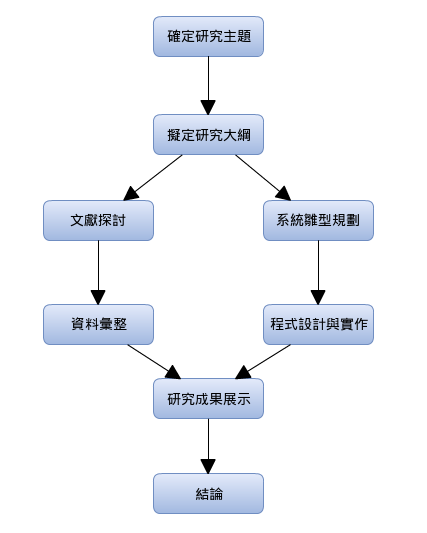
\includegraphics[width=17cm,keepaspectratio]{ch2/研究流程圖.png}
\caption{\label{fig:研究流程圖}研究流程圖}
\end{figure}

  \section{研究對象}
我們這組的研究對象就是學校以及學生,因為臺北城市科技大學有證照點數的畢業門檻,為了讓所有學生可以方便查詢自己的點數以及讓學校方便管理所以我們才會有這個想法。

\chapter{文獻回顧}

\subsection{寫作提示} 
1.文獻評論主要是在作者先搞清楚自己所欲探討之主題與相關問題後,針對自己所
欲探討之主題與相關問題,到底在中西方既存研究文獻中,已有那些研究成果,
作者必須先搞清楚,也讓他人能很快的作重點式了解,如同「站在巨人的肩膀上」
回顧過去前瞻未來,針對該主題與相關問題進行探討。
2.文獻探討之步驟主要有四:
\begin{enumerate}[noitemsep]
\item (1)歸類:將類似的文獻歸於一類,此部分可根據自己的標準來進行歸類。
\item (2)摘要:以往文獻勢不可能全文摘錄,因此必須根據過去文獻的重點進行摘要。

通常重要的資訊包括研究的年代、研究的對象、研究的方法以及研究的結論等。
\item (3)批判:在整理完過去文獻之後,必須對相關文獻進行檢討,了解過去文獻研究所不足之處,作為未來研究的改進方向。
\item (4)建議:即前述所說明的未來改進方向,最好該建議改進方向就是自己研究所欲加強之處。
\end{enumerate}

3.相關理論之探討與說明
(1)說明與研究題目有關且與欲探索之研究問題頗具相關之理論為何種理論,可簡
列數 個,並以一個段落說明即可。
(2)針對所欲探討之題目與欲研究問題最具相關性,且作者最感興趣的某一個理論
詳加討論。
4.文獻評論之最後段落,宜針對前人之研究成果所採用之研究途徑、方法作一檢
討,並說明其優缺點,進而針對作者所欲探討之主題與相關問題,作者自認宜先
採用何種研究途徑,再採取何種研究方法,以利突顯自己的研究方法,有別於他
人。

  \section{相關技術}
本項研究使用MySQL資料庫,用PHP來引導資料庫呈現搜尋資訊、用Dreamweaver來開發網頁環境、Apache HTTP Server架設伺服器、用Photoshop影像處理修圖與繪圖,使用HTML、 CSS 、JavaScript來寫程式碼編輯網頁裡的內容、邊框的處理、顏色的調配、文字內容以及連結、排版和編輯學生考到證照的點數以及名稱。

  \section{專案特性}

下層分級(IaaS):雲端設備將基礎硬體設備整合起來透過網路,像旅館一樣,分隔成不同的房間供企業租用,資訊科技管理人員可以透過網路存取運算能力或儲存空間。

中層分級(PaaS):雲端平台打造程式開發平台與作業系統平台,讓開發人員可以透過網路撰寫程式與服務,一般消費者也可以在上面執行程式。

上層分級(SaaS):雲端軟體將軟體應用透過網路以訂閱的方式提供服務,使用者可以隨時隨地存取各項服務。所有人都可以在上面自由揮灑創意,提供各式各樣的迎合市場的服務。

  \section{學生證照管理系統功能介紹}

\begin{enumerate}[noitemsep]
\item 證照查詢功能:
對於已註冊的會員可查詢資管專業技術證照相關資訊。
例如:最近一場考試的時間地點。

\item 後端平台管理功能:
系統管理者可以有權限刪除資料庫的資料,發佈最新消息。
例如:公佈證照獎金申請開始消息…等。

\item 學生證照影像檔的存儲功能:
學生可上傳已考取的證照影本,當學校要求系上提供證照影本等佐證資料時,可以快速提供。
此外,原本系上證照影本的管理是以資料夾的方式,由於此方式不僅佔空間,而且當要特別找某ㄧ位同學的證照時,更是ㄧ件麻煩的事情,使用電子方式存放證照影本,應可解決以上問題。

\item 與學校行政系統資料庫格式相容:
系統可以輸出與學校行政系統資料庫格式相容的輸出檔,以方便學校後續的作業。

\item 證照統計結果展示:
系統會根據所設定的搜尋條件,以網頁呈現統計結果。
例如:可顯現歷年來學生考過的證照張數,並提供友善列印的功能。

\item 報表輸出:
由於學校常有各式各樣的資料需求。
例如:校務基本資料表與獎補助款申請資料表,本系統預計開發報表輸出功能,只要設定所需的報表類型,按下一個按鈕就可以輸出學校所要的格式,以減少人工作業的時間。
\end{enumerate}

  \section{關鍵因素成功之定義}
    
對於一般人而言,雲端運算裡面所說的「雲」是虛無飄渺的詞彙而已,但往往多數人卻忽略這一項基本需求,以至於用戶端無法感受「有雲」及「無雲」間的差異性,但雲端運算對於企業、社交環境卻有著很大的影響。

對於雲端運算而言最佳的網路架構,就是能夠提供高彈性、高可用性且高適應性,經過技術論證及實例探討之後,有五大步驟是確保雲端運算導入成功的關鍵,分別是分割、集中化、匯集、自動化、自由化。 
     
目前市場上「雲端運算」,最常看到的IaaS、PaaS及SaaS三項發展方向,資訊科技基礎設施、資訊發展平台及資訊應用服務三項作一妥善整合,提供組員內的人員更好的資訊及使用環境,且間接提升組員的能力。因學校學生人數眾多,常常許多人一起登入時會導致學校系統故障,又或者是當機或登不進去的現象,所以本項研究想要從原本固定式網路架構成功轉移成雲端運算時,就不再需要為了臨時出現的尖峰流量或服務需求,預先規劃並建置過高的相關設備;而能夠以動態方式,適度轉移其他系統的能量以因應所需。
   
在雲端的運算服務裡面通常都具備幾項成功的特徵:

\begin{enumerate}[noitemsep]
\item 採用虛擬化的技術,能夠快速上傳資料或取得服務
\item 透過網路的提供,可以處理龐大的資料
\item 減少使用者對終端機處理資料的負擔
\item 使用者可以隨時隨地的加入與參與
\item 具可以高度伸縮的擴充功能
\item 降低使用者對於資訊科技專業知識的依賴
\item 按照使用量付費,對使用者需求提供資源
\end{enumerate}


  \section{成功個案研討}

本項研究成功的個案是國立屏東科技大學技術證照系統如圖 \ref{fig:屏科大} 所示,此系統主要負責證照管理,包含學生取得證照獎勵方法、專業證照獎勵標準表、證照審核流程圖、獎勵金流程圖。此校全力推動提升學生考取證照意願之作業,且配合各行政單位個別需求,開發各項管理系統以達到提昇考取證照意願與教學服務水準。

技術證照系統網路業務

\begin{enumerate}[noitemsep]
\item 建立跟整合證照資訊的系統
\item 管理系統介面與內容設計和分析
\item 管理證照系統分析與設計
\item 處理證照點數排行
\item 規劃技術證照系統 
\end{enumerate}

\begin{figure}[h]
\centering 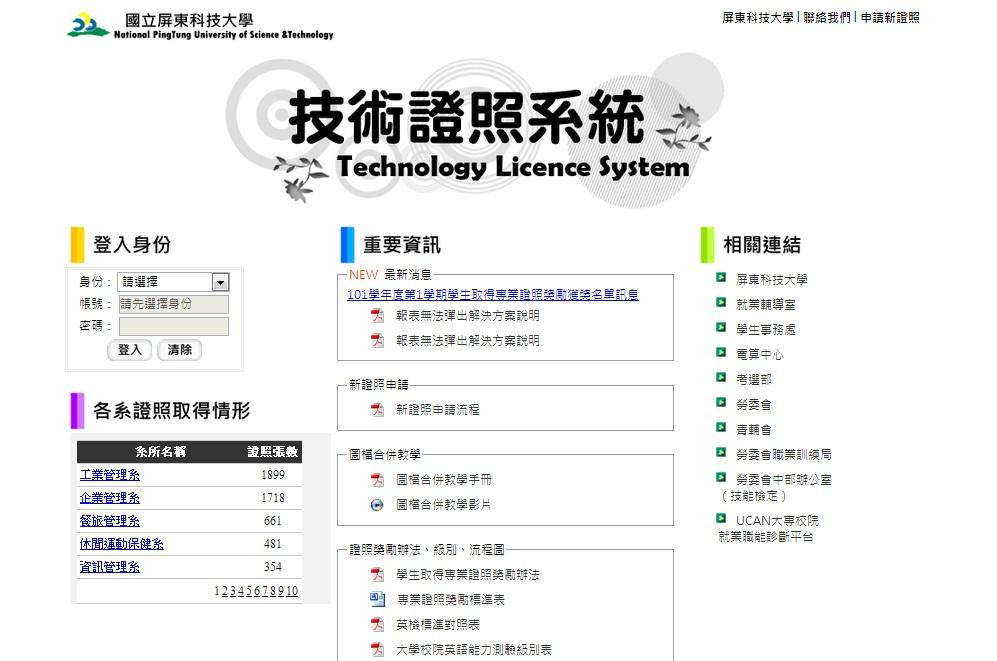
\includegraphics[width=18cm,keepaspectratio]{ch2/2.1.jpg}
\caption{\label{fig:屏科大}國立屏東科技大學技術證照系統登入介面}
\end{figure}


\chapter{網站應用程式系統實作}

  \section{研究方法論}
本項研究採用了生命週期法,此法可以強調系統的整體性,並採用自頂向下的原則分析與設計系統,先解決全局問題並強調系統整體優化的前提下,來考慮具體的解決方案,而這個方法也稱SDLC法,並且有以下數種特點:
\begin{enumerate}[noitemsep]
\item 生命週期的階段定義分明和嚴謹的專案管理控制;
\item 前一階段完成,方可進行下一階段之工作;
\item 每個階段必有其一定的程序並力求完整、正確、嚴謹;
\item 使用者僅在分析與系統測試時參與、且用於大型複雜系統與專案所需;
\item 分析設計嚴謹、品質好、效率好;
\item 按部就班且為循序漸進的過程
\end{enumerate}

生命週期法的五個階段:
\begin{enumerate}[noitemsep]
\item 劃定系統開發範圍:定義組織所要解決的問題,策畫項目開發的範圍和制訂項目開發的計劃;
\item 系統分析:定義新系統的邏輯需求,建立邏輯模型;
\item 系統設計:滿足系統分析階段所定義的用戶的邏輯需求轉換為設計說明;
\item 系統實施:把書面上設計的系統變為可以運行的軟體系統;
\item 系統支持:系統在正式運行後,需要對其進行日常運行之管理,並對系統進 行修改和完善,一般將其稱為系統支持。
\end{enumerate}


  \section{研究設計}

本研究建置之雲端資料庫,依照用途可分為兩部份,第一部分由使用者系統所組成,主要用於學生證照管理系統,可以對資料進行新增、修改、查詢等操作;第二部份則由管理者系統所組成,主要用來開啟「學生證照管理系統」的管理者後台系統。

EER 架構圖如圖 \ref{fig:eer} 所示。

\begin{figure}[!h]
\centering 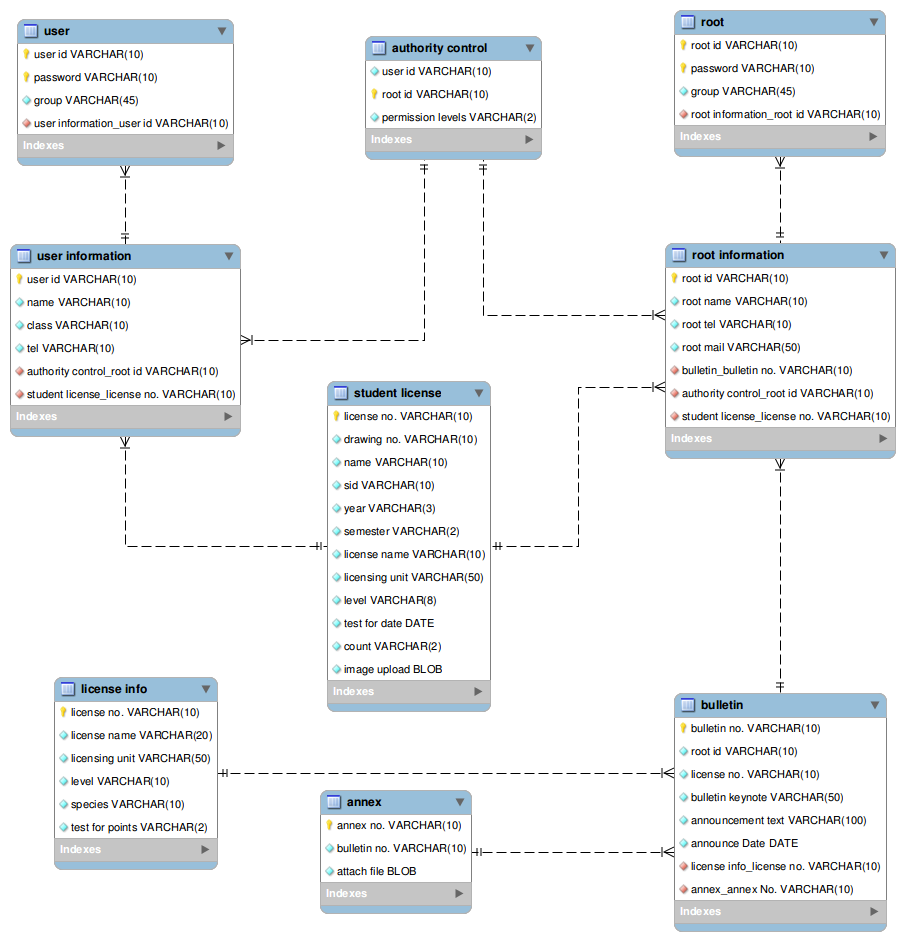
\includegraphics[width=17cm,keepaspectratio]{ch3/eer.png}
\caption{\label{fig:eer}EER 架構圖如圖}
\end{figure}

  \section{資料庫欄位表格說明}

\begin{table}[H]
\caption{使用者 (user)}
\label{tab:使用者}
\renewcommand{\arraystretch}{1} % 將表格行間距加大為原來的 1 倍
\arrayrulewidth=0.5pt               % 調整線條粗細為 1pt
%\tabcolsep=60pt                   % 調整欄間距為 24pt
\centering
\begin{tabular}[t]{|c|c|c|c|c|c|}  % 第一欄位使用 sans serif 字族
\hline
編號 & 欄位名稱 & 欄位英文 & 型態 & 長度 & 屬性 \\
\hline
A.1 & 使用者帳號 ID & user id & varchar & 10 & PK \\
\hline
A.2 & 使用者密碼 & password & varchar & 10 & PK \\
\hline
& 群組 & group & varchar & 10 &  \\
\hline
\end{tabular}
\end{table}

\begin{table}[H]
\caption{使用者基本資料(user information)}
\label{tab:使用者基本資料}
\renewcommand{\arraystretch}{0.9} % 將表格行間距加大為原來的 1 倍
\arrayrulewidth=0.5pt               % 調整線條粗細為 1pt
%\tabcolsep=60pt                   % 調整欄間距為 24pt
\centering
\begin{tabular}[t]{|c|c|c|c|c|c|}  % 第一欄位使用 sans serif 字族
\hline
編號 & 欄位名稱 & 欄位英文 & 型態 & 長度 & 屬性 \\
\hline
A.1.1 & 使用者帳號 ID & user id & varchar & 10 & PK \\
\hline
& 學生姓名 & name & varchar & 10 & \\
\hline
& 班級 & class & varchar & 10 & \\
\hline
& 聯絡電話 & tel & varchar & 10 & \\
\hline
& 學生信箱 & email & varchar & 50 & \\
\hline
\end{tabular}
\end{table}

\begin{table}[H]
\caption{管理者 (root)}
\label{tab:管理者}
\renewcommand{\arraystretch}{1} % 將表格行間距加大為原來的 1 倍
\arrayrulewidth=0.5pt               % 調整線條粗細為 1pt
%\tabcolsep=60pt                   % 調整欄間距為 24pt
\centering
\begin{tabular}[t]{|c|c|c|c|c|c|}  % 第一欄位使用 sans serif 字族
\hline
編號 & 欄位名稱 & 欄位英文 & 型態 & 長度 & 屬性 \\
\hline
B.1 & 管理者帳號 & root id & varchar & 10 & PK \\
\hline
B.1 & 管理者密碼 & root password & varchar & 10 & PK \\
\hline
& 群組 & group & varchar & 10 & \\
\hline
\end{tabular}
\end{table}

\begin{table}[H]
\caption{管理者基本資料(root information)}
\label{tab:管理者基本資料}
\renewcommand{\arraystretch}{1} % 將表格行間距加大為原來的 1 倍
\arrayrulewidth=0.5pt               % 調整線條粗細為 1pt
%\tabcolsep=60pt                   % 調整欄間距為 24pt
\centering
\begin{tabular}[t]{|c|c|c|c|c|c|}  % 第一欄位使用 sans serif 字族
\hline
編號 & 欄位名稱 & 欄位英文 & 型態 & 長度 & 屬性 \\
\hline
B.1.1 & 管理者帳號 ID & user id & varchar & 10 & PK \\
\hline
& 管理者姓名 & root name & varchar & 10 & \\
\hline
& 管理者電話 & root tel & varchar & 10 & \\
\hline
& 管理者信箱 & root email & varchar & 50 & \\
\hline
\end{tabular}
\end{table}

\begin{table}[H]
\caption{權限控制資料(authority control)}
\label{tab:權限控制資料}
\renewcommand{\arraystretch}{1} % 將表格行間距加大為原來的 1 倍
\arrayrulewidth=0.5pt               % 調整線條粗細為 1pt
%\tabcolsep=60pt                   % 調整欄間距為 24pt
\centering
\begin{tabular}[t]{|c|c|c|c|c|c|}  % 第一欄位使用 sans serif 字族
\hline
編號 & 欄位名稱 & 欄位英文 & 型態 & 長度 & 屬性 \\
\hline
C.1 & 使用者帳號 & user id & varchar & 10 & FK \\
\hline
C.2 & 管理者帳號 & root id & varchar & 10 & PK \\
\hline
C.3 & 權限級別 & permission levels & varchar & 2 & \\
\hline
\end{tabular}
\end{table}

\begin{table}[H]
\caption{學生證照資料(student license)}
\label{tab:學生證照資料}
\renewcommand{\arraystretch}{1} % 將表格行間距加大為原來的 1 倍
\arrayrulewidth=0.5pt               % 調整線條粗細為 1pt
%\tabcolsep=60pt                   % 調整欄間距為 24pt
\centering
\begin{tabular}[t]{|c|c|c|c|c|c|}  % 第一欄位使用 sans serif 字族
\hline
編號 & 欄位名稱 & 欄位英文 & 型態 & 長度 & 屬性 \\
\hline
D.1 & 證照編號 & license no. & varchar & 10 & FK \\
\hline
D.2 & 圖檔編號 & drawing no. & varchar & 10 & FK \\
\hline
D.3 & 姓名 & name & varchar & 10 & \\
\hline
D.4 & 學號 & sid & varchar & 10 & \\
\hline
D.5 & 班級 & class & varchar & 10 & \\
\hline
D.6 & 考取學年 & year & varchar & 3 & \\
\hline
D.7 & 考取學期 & semester & varchar & 2 & \\
\hline
D.8 & 證照名稱 & license name & varchar & 10 & \\
\hline
D.9 & 發照單位 & licensing unit & varchar & 50 & \\
\hline
D.10 & 級別 & level & varchar & 10 & \\
\hline
D.11 & 考照日期 & test for date & date & 8 & \\
\hline
D.12 & 證照點數 & count & varchar & 2 & \\
\hline
D.13 & 圖片上傳 & image upload & blob & & \\
\hline
\end{tabular}
\end{table}


\begin{table}[H]
\caption{公佈欄資料(bulletin)}
\label{tab:公佈欄資料}
\renewcommand{\arraystretch}{1} % 將表格行間距加大為原來的 1 倍
\arrayrulewidth=0.5pt               % 調整線條粗細為 1pt
%\tabcolsep=60pt                   % 調整欄間距為 24pt
\centering
\begin{tabular}[t]{|c|c|c|c|c|c|}  % 第一欄位使用 sans serif 字族
\hline
編號 & 欄位名稱 & 欄位英文 & 型態 & 長度 & 屬性 \\
\hline
E.1 & 公佈欄編號 & bulletin no. & varchar & 10 & PK \\
\hline
E.2 & 管理者帳號 & root id & varchar & 10 & FK \\
\hline
E.3 & 證照編號 & license no. & varchar & 10 & FK \\
\hline
E.4 & 公佈欄主旨 & bulletin keynote & varchar & 50 & \\
\hline
E.5 & 公佈內文 & announcement text & varchar & 100 & \\
\hline
E.6 & 公佈日期 & announce date & date & 8 & \\
\hline
\end{tabular}
\end{table}

\begin{table}[H]
\caption{附件(annex)}
\label{tab:附件}
\renewcommand{\arraystretch}{1} % 將表格行間距加大為原來的 1 倍
\arrayrulewidth=0.5pt               % 調整線條粗細為 1pt
%\tabcolsep=60pt                   % 調整欄間距為 24pt
\centering
\begin{tabular}[t]{|c|c|c|c|c|c|}  % 第一欄位使用 sans serif 字族
\hline
編號 & 欄位名稱 & 欄位英文 & 型態 & 長度 & 屬性 \\
\hline
F.1 & 附件編號 & annex no. & varchar & 10 & PK \\
\hline
F.2 & 公佈欄編號 & bulletin no. & varchar & 10 & FK \\
\hline
F.3 & 附加檔案 & attach file & text & 20MB &  \\
\hline
\end{tabular}
\end{table}

\begin{table}[H]
\caption{證照資訊(license info)}
\label{tab:證照資訊}
\renewcommand{\arraystretch}{1} % 將表格行間距加大為原來的 1 倍
\arrayrulewidth=0.5pt               % 調整線條粗細為 1pt
%\tabcolsep=60pt                   % 調整欄間距為 24pt
\centering
\begin{tabular}[t]{|c|c|c|c|c|c|}  % 第一欄位使用 sans serif 字族
\hline
編號 & 欄位名稱 & 欄位英文 & 型態 & 長度 & 屬性 \\
\hline
G.1 & 證照編號 & license no. & varchar & 10 & PK \\
\hline
G.2 & 證照名稱 & license name & varchar & 20 &  \\
\hline
G.3 & 級別 & level & varchar & 10 & \\
\hline
G.4 & 種類 & species & varchar & 5 & \\
\hline
G.5 & 發照單位 & licensing unit & varchar & 50 & \\
\hline
G.6 & 證照點數 & count & varchar & 2 & \\
\hline
\end{tabular}
\end{table}

\begin{figure}[h]
\centering 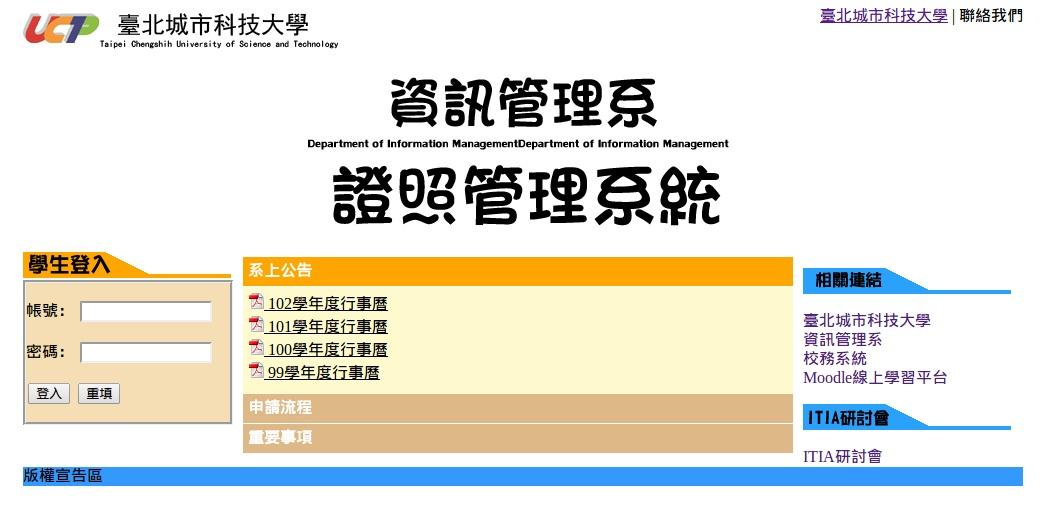
\includegraphics[width=17cm,keepaspectratio]{ch3/login}
\caption{\label{fig:login}學生證照管理系統登入與使用介面}
\end{figure}

\begin{figure}[h]
\centering 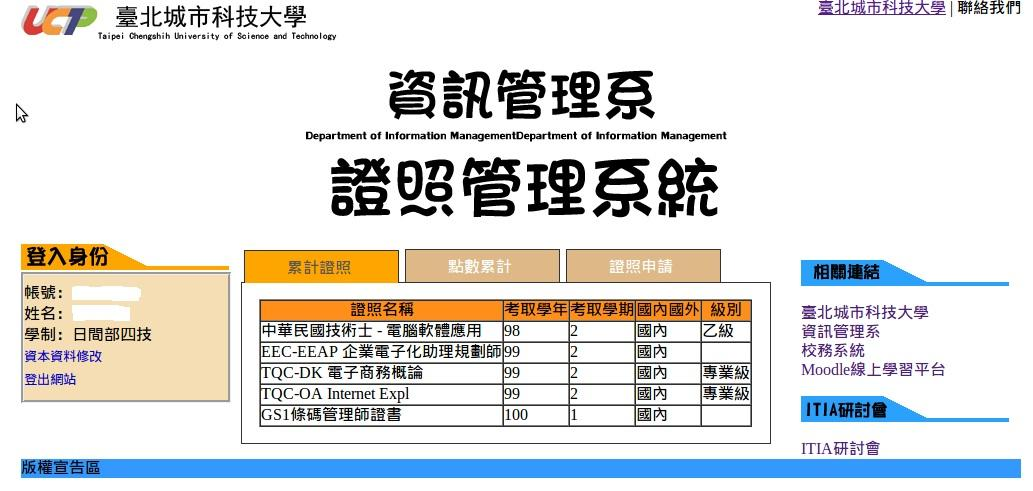
\includegraphics[width=17cm,keepaspectratio]{ch3/homepage}
\caption{\label{fig:homepage}學生證照管理系統使用介面圖}
\end{figure}

  \section{研究設備}

本項研究所使用的 Ubuntu 作業系統,核心系統為 Linux,此作業系統最大特色硬體支援性佳、簡單的安裝過程、友善的操作環境、豐富的軟體套件,系統的特色為開放原始碼和執行速度快、配備需求低、核心功能強大穩定、獨立作業、免費或是少許的費用、安全性高、發現漏洞時可執行快速修復、多功能、多使用者、使用者與群組的規劃、相對比較不耗費資源系統、適合只需要小核心的嵌入式系統。開發工具軟體均是免費使用的,開發者可以使用 HTML、 CSS 、JavaScript 程式碼來開發網頁裡的內容。

本項研究也使用 Dreamweaver 做為開發網頁環境,Apache HTTP Server 架設伺服器,MySQL 資料庫,用 PHP 來引導資料庫呈現搜尋資訊,開發環境的作業系統為 Windows 7 x64 位元、x86 位元,網路服務平台的作業系統為Microsoft Windows Server 2013 x64、x86。詳細的研究開發環境如表 \ref{tab:系統開發環境平台及工具} 系統開發環境平台及工具所示。

\begin{table}[!t]
\caption{系統開發環境平台及工具}
\label{tab:系統開發環境平台及工具}
\renewcommand{\arraystretch}{1} % 將表格行間距加大為原來的 1 倍
\arrayrulewidth=0.5pt               % 調整線條粗細為 1pt
%\tabcolsep=60pt                   % 調整欄間距為 24pt
\centering
\begin{tabular}[t]{|c|c|}  % 第一欄位使用 sans serif 字族
\hline
項目 & 規格 \\
\hline
服務管理平台 & Windows 7 x64、x86 \\
\hline
開發環境 & Dreamweaver、Apache HTTP Server \\
\hline
使用程式語言 & HTML、 CSS 、JavaScript \\
\hline
使用繪圖軟體 & Photoshop \\
\hline
學生資料查詢 & MySQL、PHP \\
\hline
\end{tabular}
\end{table}

\chapter{作品展示}

待撰寫

\chapter{建議與結論}

待撰寫

\chapter{\LaTeX 排版技巧}

  \section{程式碼展示}

這裡介紹在 \LaTeX 中,如何將程式碼的呈現方式。

研究自行開發的程式庫(Layout Library) ..... 如 \ref{list:sample1}

    \noindent \begin{minipage}[t]{1\textwidth} \lstinputlisting[language=tex,
      caption={程式碼模式展示}, 
      label=list:sample1]
      {code/sample.html}
    \end{minipage}

  \section{\LaTeX 的表格製作}

這裡介紹在 \LaTeX 中,如何呈現表格。

建立一個指定寬的的表格,如表 \ref{tab:table1} 所示。

\begin{table}[htbp]
\centering
\caption{\label{tab:table1}指定寬度與高度的表格}
\begin{tabular}{|p{3cm}|p{3cm}|}
\hline
格子 1 & 格子 2 \\[1cm]
\hline
\multicolumn{2}{|l|}{格子 3} \\[2cm]
\hline
格子 4 & 格子 5 \\[1cm]
\hline
\end{tabular}
\end{table}

建立一個表格內容置中,合併儲存格,如表 \ref{tab:table1} 所示。

\begin{table}[htbp]
\centering
\caption{\label{tab:table2}表格內容置中,合併儲存格}
\begin{tabular}{|c|c|c|c|c|}
\hline
\multirow{2}{*}{Multi-Row} &
\multicolumn{2}{c|}{Multi-Column} &
\multicolumn{2}{c|}{\multirow{2}{*}{Multi-Row and Col}} \\
\cline{2-3}
  & column-1 & column-2 & \multicolumn{2}{c|}{} \\
\hline
label-1 & label-2 & label-3 & label-4 & label-5 \\
\hline
\end{tabular}
\end{table}


% \input{chapter2}
% \input{chapter3}
% \input{chapter4}
% \input{chapter5}

%\input{chap_last}

%%% 參考文獻
\newpage
\baselineskip=20pt
\phantomsection % for hyperref to register this
\addcontentsline{toc}{chapter}{\nameRef}
\renewcommand{\bibname}{\protect\makebox[5cm][s]{\nameRef}}
%  \makebox{} is fragile; need protect
\bibliographystyle{ieeetr}  % 使用 IEEE Trans 期刊格式
%\bibliography{my_bib}

\begin{thebibliography}{1}
\bibitem{a-comparison-of-mvx-framework}
A Comparison of Angular, Backbone, CanJS and Ember, http://sporto.github.io/blog/2013/04/12/comparison-angular-backbone-can-ember/, [Online; accessed Jun-17-2013]. 

\bibitem{html-as-it-should-be}
AngularJS - HTML as it should be, https://www.slidecaptain.com/flows/5176d0f60b42f0ed700007f4 [Online; accessed Jun-27-2013]. 

\bibitem{angularjs.org}
AngularJS by Google, http://angularjs.org/, [Online; accessed Jun-17-2013]. 

\bibitem{AngularJS-is-MVW}
AngularJS to be MVW framework, https://plus.google.com/+AngularJS/posts/aZNVhj355G2, [Online; accessed Jun-07-2013]. 

\bibitem{wiki-AngularJS}
AngularJS, http://en.wikipedia.org/wiki/AngularJS, [Online; accessed Jun-07-2013]. 

\bibitem{paper: webapp using mvc}
Avraham Leff and James T. Rayfield, "Web-Application Development Using the ModelNiewlController Design Pattern", Fifth IEEE International Conference on Enterprise Distributed Object Computing, 2001, pp 118-127. 

\bibitem{CodeIgniter}
CodeIgniter, https://zh.wikipedia.org/wiki/CodeIgniter, [Online; accessed Jun-27-2013]. 

\bibitem{CodeIgniter-Flow-Chart}
CodeIgniter Application Flow Chart, http://ellislab.com/codeigniter/user-guide/overview/appflow.html, [Online; accessed Jun-27-2013]. 

\bibitem{Codeigniter-Tutorial}
Codeigniter Tutorial, http://www.revillwebdesign.com/codeigniter-tutorial/, [Online; accessed Jun-17-2013]. 

\bibitem{data-binding-in-angular}
Data Binding in Angular, http://docs.angularjs.org/guide/dev\_guide.templates.databinding, [Online; accessed Jun-17-2013]. 

\bibitem{Data-binding}
Data-binding, http://en.wikipedia.org/wiki/Data\_binding, [Online; accessed Jun-17-2013]. 

\bibitem{wiki-back-and-front-end}
Front and back ends, http://en.wikipedia.org/wiki/Front\_and\_back\_ends, [Online; accessed Jun-17-2013]. 

\bibitem{wiki-git}
Git, https://en.wikipedia.org/wiki/Git\_(software), [Online; accessed Jun-17-2013]. 

\bibitem{site: github}
Github, https://github.com/, [Online; accessed Jun-17-2013]. 

\bibitem{JavaScript}
JavaScript, https://zh.wikipedia.org/wiki/JavaScript, [Online; accessed Jun-17-2013]. 

\bibitem{paper-MVP-for-C-Java}
M. Potel. "MVP: Model-View-Presenter — The Taligent Programming Model for C++ and Java", Taligent, Inc, 1996, 16 pages. 

\bibitem{wiki-MVC}
MVC, http://zh.wikipedia.org/wiki/MVC, [Online; accessed Jun-17-2013]. 

\bibitem{MVP-MVC-MVVM}
MVP, MVC, MVVM, 傻傻分不清楚, http://www.dotblogs.com.tw/regionbbs/archive/2011/09/29/compare.to.mvp.mvc.mvvm.aspx, [Online; accessed Jun-17-2013] 

\bibitem{wiki-MVVM}
MVVM, http://en.wikipedia.org/wiki/Model\_View\_ViewModel, [Online; accessed Jun-17-2013]. 

\bibitem{MVC-history}
Model View Controller History, ParcPlace(move from Xerox Parc), http://c2.com/cgi/wiki?ModelViewControllerHistory, [Online; accessed Jun-17-2013]. 

\bibitem{wiki-php}
PHP, https://zh.wikipedia.org/zh-tw/PHP, [Online; accessed Jun-17-2013]. 

\bibitem{book: JavaScript Patterns}
Stoyan Stefanov, "JavaScript Patterns", O'Reilly Media, September 28, 2010. 

\bibitem{cookbook-using-MVC}
lenn E. Krasner and Stephen T. Pope, "A cookbook for using the model-view controller user interface paradigm in smalltalk-80", Journal Of Object Oriented Programming, vol.1 Issue 3, pp.26-49, Aug./Sept 1988. 

\bibitem{wiki-web-programming}
動態網頁, https://zh.wikipedia.org/wiki/動態網頁, [Online; accessed Jun-17-2013]. 
\end{thebibliography}


\clearpage
%\end{CJK}
\end{document}
